\documentclass{beamer}
\usepackage[spanish]{babel}
\usepackage[utf8]{inputenc}
\usepackage{graphics}
\usepackage{amssymb} % Simbolos matematicos
\usepackage{moreverb} 
\usepackage{listings} % Para listar código

% imprimir
% \documentclass[handout]{beamer} 
% \usepackage{pgfpages}
% \pgfpagesuselayout{4 on 1}[a4paper,landscape,border shrink=5mm]

\mode<presentation> {
  \usetheme{Singapore}
%  \usetheme{Bergen}
  \useoutertheme{infolines}
  %\useoutertheme[]{miniframes}
  \usefonttheme{structurebold}
  \setbeamercovered{transparent}
}

\setbeamertemplate{headline}
{%
  
\includegraphics[height=1.5cm]{format/eoi-header.jpg}%
}

\setbeamercolor{titlelike}{fg=white}
\setbeamercolor{frametitle}{fg=black}

%% Metadatos del PDF.
\hypersetup{  
  pdftitle={GnuPG},
  pdfauthor={Miguel Vidal, Israel Herraiz},
%  pdfcreator={GSyC/Libresoft},
  pdfproducer=PDFLaTeX,
  pdfsubject={Máster EOI (Area TIC)},
}
%%

%\setbeamerfont*{frametitle}{size=\huge}

\defbeamertemplate*{footline}{shadow theme}
{%
  \leavevmode%
  \hbox{\begin{beamercolorbox}[wd=.5\paperwidth,ht=2.5ex,dp=1.125ex,leftskip=.1cm plus1fil,rightskip=.2cm]{author in head/foot}%

\includegraphics[scale=0.40]{format/cc-by-80x15.png} \hspace{0.05cm}
	Miguel Vidal / Israel Herraiz
  \end{beamercolorbox}%
  \begin{beamercolorbox}[wd=.5\paperwidth,ht=2.5ex,dp=1.125ex,plus1fil]{title in head/foot}%
    \usebeamerfont{title in head/foot}\insertshorttitle \hspace{0.5cm} %
	\hspace{0.2cm}  01/10/2011 \hspace{0.2cm}
    \usebeamerfont{author in head/foot}\insertframenumber\,/\,\inserttotalframenumber
  \end{beamercolorbox}}%
  \vskip0pt%
}


\begin{document}

\title{Cifrado y firma digital con GnuPG}
\subtitle{Máster en Economía Digital e Industrias Creativas}
% \author{Miguel Vidal\thanks{\small{ETSI de Telecomunicación, URJC}} \\ Departamento de Sistemas Telemáticos y Computación.
% \and 
% Israel Herraiz\thanks{ETSI Caminos, UPM} \\ Departamento de Matemáticas e Informática.}  
% 
\date{\footnotesize{1 de octubre de 2011}}
\author{Miguel Vidal \hspace{1cm} Israel Herraiz \\
{\tiny ETSIT, URJC \hspace{1,9cm} ETSICCP, UPM} \\
\hspace{-0.4cm} {\tiny Twitter: @mvidallopez \hspace{1.5cm}Twitter: @herraiz}
}


{
\frame{
\setbeamercolor{titlelike}{fg=red}
\maketitle
\begin{center}
\vspace{-0.5cm}

\includegraphics[width=3cm]{format/urjc}
\hspace{1cm}

\includegraphics[width=1.8cm]{format/upm}
\end{center}
}
}

\frame{
~
\vspace{2cm}

\begin{footnotesize}
\begin{flushright}
  \copyright~ 2011 Miguel Vidal, Israel Herraiz \\
\medskip
  Este artículo se distribuye bajo licencia \\
 ``Reconocimiento 3.0 España'' de Creative Commons. \\
\smallskip 
    \href{http://creativecommons.org/licenses/by/3.0/es}{
\includegraphics[width=2cm]{format/cc-by.png}} \\
    {\tiny \url{http://creativecommons.org/licenses/by/3.0/es}}
\end{flushright}
\end{footnotesize}

}
%%

\usebackgroundtemplate{}

\AtBeginSubsection[]
{
  \begin{frame}<beamer>{Índice}
    \tableofcontents[currentsection,currentsubsection]
  \end{frame}
}



%%%%%%%%%%%%%%%%%%%%%%%%%%%%%%%%%%%%%%%%%%%%%%%%%%%%%%%%%%%%%%%%%%%%%%%
\section{PGP, OpenPGP, GnuPG}
%%%%%%%%%%%%%%%%%%%%%%%%%%%%%%%%%%%%%%%%%%%%%%%%%%%%%%%%%%%%%%%%%%%%%%%

\subsection{PGP}
%%%%%%%%%%%%%%%%%%%%%%%%%%%%%%%%%%%%%%%%%%%%%%%%%%%%%%%%%%%%%%%%%%%%%%%

\begin{frame}
\frametitle{¿Qué es PGP?}

\begin{itemize}
\item \alert{Pretty Good Privacy}: primera implementación popular del cifrado de clave pública (RSA).
\item Creado en solitario por Phil Zimmermann en 1991, un activista de los ciberderechos. 
\item Lo puso a disposición de todo el mundo (código fuente incluido) vía FTP.
\item Se popularizó rápidamente y recibió caluroso apoyo de la comunidad de criptógrafos para la versión 2.0 (1992).
\end{itemize}

\end{frame}

%%%%%%%%%%%%%%%%%%%%%%%%%%%%%%%%%%%%%%%%%%%%%%%%%%%%%%%%%%%%%%%%%%%%%%%

\begin{frame}
\frametitle{¿Qué es PGP? (2)}

\begin{itemize}
\item Zimmermann tuvo muchos problemas con la patente de RSA y fue investigado por presunta violación de las leyes de exportación de armas.
\item Su caso fue finalmente archivado en 1996.
\item Creó entonces una compañía (PGP Inc.) para explotar comercialmente PGP.
\item La patente RSA expiró en septiembre del 2000.
\item PGP Inc. fue adquirida por NAI y luego por PGP Corporation.
\end{itemize}

\end{frame}


%%%%%%%%%%%%%%%%%%%%%%%%%%%%%%%%%%%%%%%%%%%%%%%%%%%%%%%%%%%%%%%%%%%%%%%
\subsection{OpenPGP}

\begin{frame}
\frametitle{OpenPGP}

\begin{itemize}
\item Estándar abierto para PGP propuesto por Zimmermann. 
\item Aceptado por la IETF en 1998.
\item RFC 4880 (noviembre 2007), sucesor del RFC 2440.
\item Tiene muchas implementaciones, sobre todo para clientes de correo.
\item La implementación \alert{libre} de OpenPGP se llama \alert{GnuPG}.
\end{itemize}

\end{frame}

%%%%%%%%%%%%%%%%%%%%%%%%%%%%%%%%%%%%%%%%%%%%%%%%%%%%%%%%%%%%%%%%%%%%%%%
\subsection{GnuPG}
%%%%%%%%%%%%%%%%%%%%%%%%%%%%%%%%%%%%%%%%%%%%%%%%%%%%%%%%%%%%%%%%%%%%%%%


\begin{frame}
\frametitle{GnuPG}

\begin{itemize}
\item \alert{GNU Privacy Guard}: Implementación libre (GPLv3) de OpenPGP.
\item Promovido por la FSF desde 1999.
\item Fue apoyado por el Gobierno alemán en sus inicios (financiaron la documentación y el \textit{port} a Windows).
\item Se basa en interfaz de línea de comandos, con diversos \textit{frontends} gráficos.
\item Existen \textit{ports} a los sistemas operativos más utilizados (Windows, MacOS, Linux...).
\end{itemize}

\end{frame}



%%%%%%%%%%%%%%%%%%%%%%%%%%%%%%%%%%%%%%%%%%%%%%%%%%%%%%%%%%%%%%%%%%%%%%%

\begin{frame}[fragile]
\frametitle{Descargar GnuPG}

\begin{itemize}
\item Descargar e instalar GnuPG (hay versiones para Windows, MacOS, Linux, *BSD...)
	\begin{itemize}
	\item Para MacOS X, \alert{Mac GPG}: \url{http://gpgtools.org} 
	\item Para Windows, \alert{gpg4win}: \url{http://gpg4win.org}
	\end{itemize}
\item Hay GUIs: por ejemplo \alert{Seahorse} para Gnome o WPA para Windows.
\end{itemize}

\center \textit{Opcional:} podemos comprobar la integridad del fichero:

\definecolor{ivory2}{RGB}{238,238,224} % for background
% \definecolor{light-gray}{gray}{0.85}

\lstset{ 
emph={sha1sum},
emphstyle=\alert,
language=bash,
frameround=fttt,
backgroundcolor=\color{ivory2},
keywordstyle=\color{red},
commentstyle=\color{gray},
basicstyle=\normalsize,
stringstyle=\color{white},
}

\begin{lstlisting}[frame=trBL]
$ sha1sum gnupg-w32cli-1.4.10b.exe
\end{lstlisting}

\end{frame}

%%%%%%%%%%%%%%%%%%%%%%%%%%%%%%%%%%%%%%%%%%%%%%%%%%%%%%%%%%%%%%%%%%%%%%%

\begin{frame}[fragile]
\frametitle{Instalar GnuPG}

La instalación en Unix/Linux por medio del sistema de paquetes correspondiente. Por ejemplo:

\definecolor{ivory2}{RGB}{238,238,224} % for background

\lstset{ 
emph={$},
emphstyle=\color{black},
language=bash,
frame=shadowbox,
backgroundcolor=\color{ivory2},
keywordstyle=\color{red},
rulesepcolor=\color{black},
rulecolor=\color{black},
commentstyle=\color{gray},
basicstyle=\color{red}\normalsize,
stringstyle=\ttfamily,
}

\begin{lstlisting}[frame=trBL]
$ apt-get install gnupg   # Linux (Debian,Ubuntu)
$ pkg_add -vv gnupg-1.4.10p0   # OpenBSD
\end{lstlisting}

\end{frame}



%%%%%%%%%%%%%%%%%%%%%%%%%%%%%%%%%%%%%%%%%%%%%%%%%%%%%%%%%%%%%%%%%%%%%%%
\section{Gestión de claves públicas}

\begin{frame}[fragile]
\frametitle{Generar claves}

Generamos nuestro par de claves (una privada y otra pública): 

\definecolor{ivory2}{RGB}{238,238,224} % for background

\lstset{ 
emph={$},
emphstyle=\color{black},
language=bash,
frame=shadowbox,
backgroundcolor=\color{ivory2},
keywordstyle=\color{red},
rulesepcolor=\color{black},
rulecolor=\color{black},
commentstyle=\color{gray},
basicstyle=\color{red}\normalsize,
stringstyle=\ttfamily,
}

\begin{lstlisting}[frame=trBL]
$ gpg --gen-key
\end{lstlisting}

\bigskip

Nos preguntará por el algoritmo a usar (RSA), tamaño de clave (2048 bits), expiración (0), nombre real, email y comentario. \\
\medskip
También desde línea de comandos podemos pasar parámetros:
\begin{lstlisting}[frame=trBL]
$ gpg --gen-key -t rsa -b <bits 2048 o 4096>
\end{lstlisting}

\end{frame}

%%%%%%%%%%%%%%%%%%%%%%%%%%%%%%%%%%%%%%%%%%%%%%%%%%%%%%%%%%%%%%%%%%%%%%%

\begin{frame}[fragile]
\frametitle{Obtén tu key ID}

\definecolor{ivory2}{RGB}{238,238,224} % for background

\lstset{ 
emph={F724244F},
emphstyle=\alert,
language=bash,
frame=shadowbox,
backgroundcolor=\color{ivory2},
keywordstyle=\color{red},
rulesepcolor=\color{black},
rulecolor=\color{black},
commentstyle=\color{gray},
basicstyle=\normalsize,
stringstyle=\ttfamily,
}

\begin{lstlisting}[frame=trBL]

$ gpg --list-keys

/home/mvidal/.gnupg/pubring.gpg
--------------------------------------
pub 1024D/F724244F 1999-08-27
uid Miguel Vidal <mvidal@gsyc.urjc.es>
uid Miguel Vidal (URJC) <miguel.vidal@urjc.es>
uid Miguel Vidal <mvidal@computer.org>
sub 1024g/A2B68952 1999-08-27

\end{lstlisting}

\end{frame}

%%%%%%%%%%%%%%%%%%%%%%%%%%%%%%%%%%%%%%%%%%%%%%%%%%%%%%%%%%%%%%%%%%%%%%%

\subsection{Exportar clave pública}

\begin{frame}[fragile]
\frametitle{Exporta tu clave pública}

\definecolor{ivory2}{RGB}{238,238,224} % for background

\lstset{ 
emph={},
emphstyle=\alert,
language=bash,
frame=shadowbox,
backgroundcolor=\color{ivory2},
keywordstyle=\color{red},
rulesepcolor=\color{black},
rulecolor=\color{black},
commentstyle=\color{gray},
basicstyle=\color{red}\small,
stringstyle=\ttfamily,
}


Para poder enviar una clave pública a otra persona (sin usar un servidor de claves), tenemos que exportarla:
\begin{lstlisting}[frame=trBL]
$ gpg --armor --output mvidal.asc --export mvidal
\end{lstlisting}


\end{frame}

%%%%%%%%%%%%%%%%%%%%%%%%%%%%%%%%%%%%%%%%%%%%%%%%%%%%%%%%%%%%%%%%%%%%%%%

\begin{frame}[fragile]
\frametitle{Importa una clave pública}

\definecolor{ivory2}{RGB}{238,238,224} % for background

\lstset{ 
emph={},
emphstyle=\alert,
language=bash,
frame=shadowbox,
backgroundcolor=\color{ivory2},
keywordstyle=\color{red},
rulesepcolor=\color{black},
rulecolor=\color{black},
commentstyle=\color{gray},
basicstyle=\color{red}\small,
stringstyle=\ttfamily,
}


Para importar una clave pública (sin servidor de claves) a nuestro anillo de claves:
\begin{lstlisting}[frame=trBL]
$ gpg --import mvidal.gpg
\end{lstlisting}


\end{frame}



%%%%%%%%%%%%%%%%%%%%%%%%%%%%%%%%%%%%%%%%%%%%%%%%%%%%%%%%%%%%%%%%%%%%%%%

\begin{frame}[fragile]
\frametitle{Sube tu clave a un servidor de claves}

Publica tu clave en un servidor de claves:

\definecolor{ivory2}{RGB}{238,238,224} % for background

\lstset{ 
emph={},
emphstyle=\alert,
language=bash,
frame=shadowbox,
backgroundcolor=\color{ivory2},
keywordstyle=\color{red},
rulesepcolor=\color{black},
rulecolor=\color{black},
commentstyle=\color{gray},
basicstyle=\small,
basicstyle=\color{red}\small,
stringstyle=\ttfamily,
}

\begin{lstlisting}[frame=trBL]
$ gpg --keyserver pgp.rediris.es --send-keys F724244F
\end{lstlisting}

Que debe devolverte algo como:
\begin{lstlisting}[frame=trBL]
$> gpg: sending key F724244F
\end{lstlisting}

\end{frame}


%%%%%%%%%%%%%%%%%%%%%%%%%%%%%%%%%%%%%%%%%%%%%%%%%%%%%%%%%%%%%%%%%%%%%%%

\begin{frame}[fragile]
\frametitle{Descarga una clave pública}

Descarga una clave pública de un servidor de claves:

\definecolor{ivory2}{RGB}{238,238,224} % for background

\lstset{ 
emph={},
emphstyle=\alert,
language=bash,
frame=shadowbox,
backgroundcolor=\color{ivory2},
keywordstyle=\color{red},
rulesepcolor=\color{black},
rulecolor=\color{black},
commentstyle=\color{gray},
basicstyle=\small,
basicstyle=\small,
stringstyle=\ttfamily,
}

\begin{lstlisting}[frame=trBL]
gpg --keyserver pgp.rediris.es --recv-key [key_id]
\end{lstlisting}

\medskip
O también:
\begin{lstlisting}[frame=trBL]
$ gpg --keyserver pgp.rediris.es --search-keys FE0A7AF3
gpg: buscando "FE0A7AF3" de hkp servidor pgp.rediris.es
(1)	  Israel Herraiz <israel.herraiz@upm.es>
\end{lstlisting}

\end{frame}


%%%%%%%%%%%%%%%%%%%%%%%%%%%%%%%%%%%%%%%%%%%%%%%%%%%%%%%%%%%%%%%%%%%%%%%

\begin{frame}[fragile]
\frametitle{Localizar un identificador de clave pública}


¿Cómo localizo la \alert{key ID} de alguien? \\
\pause
\centering
\url{http://www.rediris.es/keyserver}

\medskip
\centering
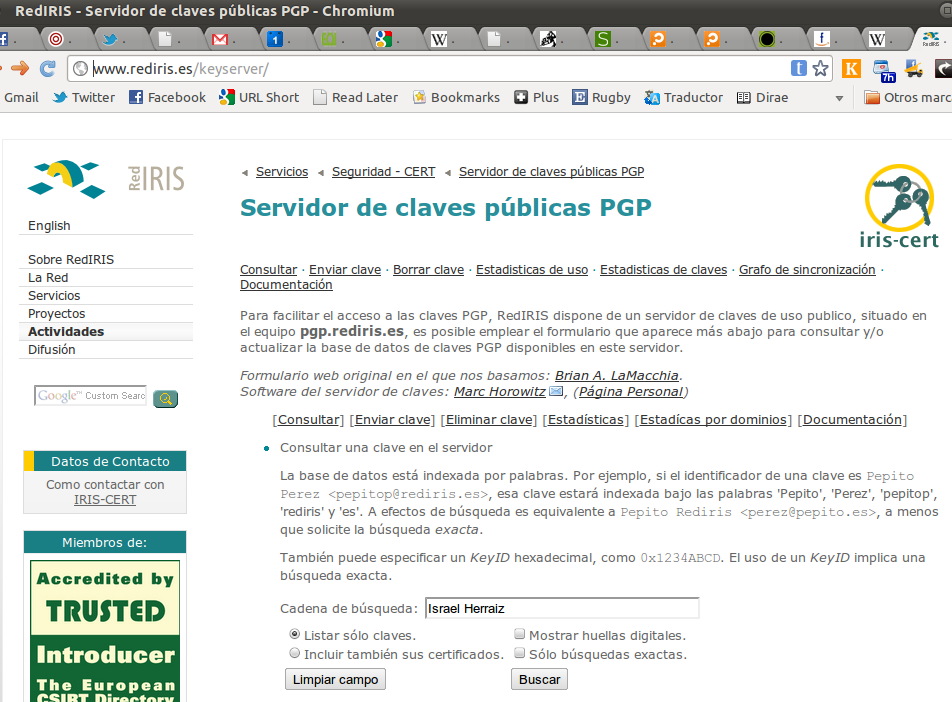
\includegraphics[scale=0.35,clip=true]{figs/rediris.png}

\end{frame}


%%%%%%%%%%%%%%%%%%%%%%%%%%%%%%%%%%%%%%%%%%%%%%%%%%%%%%%%%%%%%%%%%%%%%%%

\subsection{Firmado de claves}
\begin{frame}
\frametitle{Firmar la clave de otra persona}

\begin{enumerate}
\item Mostramos y solicitamos que se nos muestre un documento que acredite la identidad de cada cual.
\item Intercambiamos nuestras claves públicas o bien la huella digital con la persona a la que vamos a firmarle la clave (y va a firmar la nuestra). 
\item La huella digital puede entregárnosla en un papel y después podemos comprobar en nuestro ordenador que efectivamente coincide con la clave pública que poseemos de esa persona.
\item Una vez comprobado, podemos proceder a firmar su clave y otorgarle confianza.
\end{enumerate}

\end{frame}



%%%%%%%%%%%%%%%%%%%%%%%%%%%%%%%%%%%%%%%%%%%%%%%%%%%%%%%%%%%%%%%%%%%%%%%

\begin{frame}[fragile]
\frametitle{Firmar la clave de otra persona}

Descarga y comprueba las huellas y claves de tus conocidos:

\definecolor{ivory2}{RGB}{238,238,224} % for background

\lstset{ 
emph={},
emphstyle=\alert,
language=bash,
frame=shadowbox,
backgroundcolor=\color{ivory2},
keywordstyle=\color{red},
rulesepcolor=\color{black},
rulecolor=\color{black},
commentstyle=\color{gray},
basicstyle=\color{red}\small,
stringstyle=\ttfamily,
}

\begin{lstlisting}[frame=trBL]
$ gpg --keyserver pgp.rediris.es --recv-keys [key_id]
$ gpg --fingerprint [key_id]
\end{lstlisting}

\end{frame}

%%%%%%%%%%%%%%%%%%%%%%%%%%%%%%%%%%%%%%%%%%%%%%%%%%%%%%%%%%%%%%%%%%%%%%%

\begin{frame}[fragile]
\frametitle{Firmar la clave de otra persona}

Firma cada una de las claves \alert{verificadas} de tus conocidos, y súbelas al servidor de claves:

\definecolor{ivory2}{RGB}{238,238,224} % for background

\lstset{ 
emph={},
emphstyle=\alert,
language=bash,
frame=shadowbox,
backgroundcolor=\color{ivory2},
keywordstyle=\color{red},
rulesepcolor=\color{black},
rulecolor=\color{black},
commentstyle=\color{gray},
basicstyle=\color{red}\small,
stringstyle=\ttfamily,
}

\begin{lstlisting}[frame=trBL]
$ gpg --sign-key [key_id]
$ gpg --keyserver pgp.rediris.es --send-key [key_id]
\end{lstlisting}

\end{frame}


%%%%%%%%%%%%%%%%%%%%%%%%%%%%%%%%%%%%%%%%%%%%%%%%%%%%%%%%%%%%%%%%%%%%%%%

\begin{frame}
\frametitle{Observaciones}

\begin{itemize}
\item Solo se debe firmar una clave cuando se esté totalmente seguro de que dicha clave es auténtica. 
\item Esto solo puede suceder si se recibe la clave en mano. 
\item Por eso, normalmente el procedimiento de firma se realiza presencialmente.
\end{itemize}

\end{frame}

%%%%%%%%%%%%%%%%%%%%%%%%%%%%%%%%%%%%%%%%%%%%%%%%%%%%%%%%%%%%%%%%%%%%%%%

\subsection{Ejemplo de firmado de una clave}

\begin{frame}
\frametitle{Ejemplo de firmado de una clave}

\begin{block}{}
\texttt{\alert{\$ gpg --sign-key herraiz}} \\
\texttt{Orden> sign} \\
\footnotesize{\texttt{¿Está realmente seguro de querer firmar esta clave \\
con su clave: "Miguel Vidal (URJC) <miguel.vidal@urjc.es>" (F724244F)?}} \\

\medskip
\normalsize
\texttt{¿Firmar de verdad? sí} \\
\texttt{Orden> quit} \\
\texttt{¿Grabar cambios? sí} \\

\end{block}

\begin{center}
Si distribuimos nuestra clave pública, ya aparecerá con las firmas efectuadas.
\end{center}

\end{frame}

%%%%%%%%%%%%%%%%%%%%%%%%%%%%%%%%%%%%%%%%%%%%%%%%%%%%%%%%%%%%%%%%%%%%%%%

\begin{frame}
\frametitle{Resumen}

\begin{enumerate}
\item Hay que asegurarnos de que quien nos da la clave es efectivamente quien dice ser (algo imposible de verificar si nos descargamos su clave de un repositorio público o si nos la envía por email).
\item Es importante entender y mantener la consistencia de las claves de confianza (y nunca firmar si el canal por el que la hemos recibido no es fiable).
\item A diferencia de otros sistemas de criptografía de clave pública que confían en una autoridad certificadora (CA), aquí todo se basa en un \alert{sistema descentralizado} de fuentes de confianza.
\end{enumerate}

\end{frame}

%%%%%%%%%%%%%%%%%%%%%%%%%%%%%%%%%%%%%%%%%%%%%%%%%%%%%%%%%%%%%%%%%%%%%%%
\section{Cifrado}
%%%%%%%%%%%%%%%%%%%%%%%%%%%%%%%%%%%%%%%%%%%%%%%%%%%%%%%%%%%%%%%%%%%%%%%

\subsection{Cifrado con clave pública}

\begin{frame}[fragile]
\frametitle{Cifrar y descifrar un documento}

El documento que se desea cifrar es la entrada, \texttt{recipient} es el destinatario y la salida es el documento cifrado:

\definecolor{ivory2}{RGB}{238,238,224} % for background

\lstset{ 
emph={},
emphstyle=\alert,
language=bash,
frame=shadowbox,
backgroundcolor=\color{ivory2},
keywordstyle=\color{red},
rulesepcolor=\color{black},
rulecolor=\color{black},
commentstyle=\color{gray},
basicstyle=\color{red},
stringstyle=\ttfamily,
}

\begin{lstlisting}[frame=trBL]
$ gpg --output documento.gpg --encrypt --recipient \ 
        fulano@foo.es documento
\end{lstlisting}

\medskip

Para descifrar (-d):
\begin{lstlisting}[frame=trBL]
$ gpg --output documento --decrypt documento.gpg
\end{lstlisting}

\end{frame}



%%%%%%%%%%%%%%%%%%%%%%%%%%%%%%%%%%%%%%%%%%%%%%%%%%%%%%%%%%%%%%%%%%%%%%%

\subsection{Cifrado con clave simétrica}

\begin{frame}
\frametitle{Cifrado simétrico}

\begin{enumerate}
\item Funcionalidad no muy conocida de pgp/gnupg.
\item No requiere uso de clave pública ni privada.
\item Útil para cifrar ficheros para uno mismo.
\item Método rápido para usar \alert{cifrado fuerte} con usuarios que no usan gpg/pgp (mucho mejor que el cifrado fácilmente crackeable de Word o de Winzip).
\end{enumerate}

\end{frame}

%%%%%%%%%%%%%%%%%%%%%%%%%%%%%%%%%%%%%%%%%%%%%%%%%%%%%%%%%%%%%%%%%%%%%%%

\begin{frame}[fragile]
\frametitle{Cómo cifrar con clave simétrica}

\definecolor{ivory2}{RGB}{238,238,224} % for background

\lstset{ 
emph={},
emphstyle=\alert,
language=bash,
frame=shadowbox,
backgroundcolor=\color{ivory2},
keywordstyle=\color{red},
rulesepcolor=\color{black},
rulecolor=\color{black},
commentstyle=\color{gray},
basicstyle=\color{red}\small,
stringstyle=\ttfamily,
}

\begin{lstlisting}[frame=trBL]
gpg --symmetric filename
\end{lstlisting}

\medskip

Salida ASCII (para intercambiar por email):
\begin{lstlisting}[frame=trBL]
gpg --symmetric --armor filename
\end{lstlisting}

{\footnotesize(Se nos solicitará una clave: no usar la misma contraseña de nuestra clave privada.)}

\medskip

Para descifrar, se hace de la forma habitual:
\begin{lstlisting}[frame=trBL]
gpg -d filename
\end{lstlisting}


\end{frame}

%%%%%%%%%%%%%%%%%%%%%%%%%%%%%%%%%%%%%%%%%%%%%%%%%%%%%%%%%%%%%%%%%%%%%%%
\section{Firma digital}
%%%%%%%%%%%%%%%%%%%%%%%%%%%%%%%%%%%%%%%%%%%%%%%%%%%%%%%%%%%%%%%%%%%%%%%

\subsection{Firmar un documento}

\begin{frame}[fragile]
\frametitle{Firmar un documento}

El documento a firmar es la entrada y la salida es el documento firmado:

\definecolor{ivory2}{RGB}{238,238,224} % for background

\lstset{ 
emph={},
emphstyle=\alert,
language=bash,
frame=shadowbox,
backgroundcolor=\color{ivory2},
keywordstyle=\color{red},
rulesepcolor=\color{black},
rulecolor=\color{black},
commentstyle=\color{gray},
basicstyle=\color{red},
stringstyle=\ttfamily,
}

\begin{lstlisting}[frame=trBL]
gpg --armor --output document.sig --sign document
\end{lstlisting}

\medskip

Verificar la integridad de un documento firmado:
\begin{lstlisting}[frame=trBL]
gpg --verify document.sig
\end{lstlisting}

\medskip

Si además de verificar la firma queremos recuperar el documento:
\begin{lstlisting}[frame=trBL]
gpg --output document --decrypt document.sig
\end{lstlisting}


\end{frame}



%%%%%%%%%%%%%%%%%%%%%%%%%%%%%%%%%%%%%%%%%%%%%%%%%%%%%%%%%%%%%%%%%%%%%%%

{
\frame{
\setbeamercolor{titlelike}{fg=red}
\maketitle
\begin{center}

\includegraphics[width=3cm]{format/urjc}
\hspace{1cm}

\includegraphics[width=1.8cm]{format/upm}
\end{center}
}
}


\end{document}

%%%%%%%%%%%%%%%%%%%%%%%%%%%%%%%%%%%%%%%%%%%%%%%%%%%%%%%%%%%%%%%%%%%%%%%
%%%%%%%%%%%%%%%%%%%%%%%% FIN %%%%%%%%%%%%%%%%%%%%%%%%%%%%%%%%%%%%%%%%%%
%%%%%%%%%%%%%%%%%%%%%%%%%%%%%%%%%%%%%%%%%%%%%%%%%%%%%%%%%%%%%%%%%%%%%%%

Practica gpg

<ixra> 1. crear clave
<ixra> 2. subir clave
<ixra> 3. bajar clave de otros
<ixra> 4. firmar (documentos y/o claves)
<ixra> 5. subir claves de otro
<ixra> bueno, tambien quizas cifrar

%%%%%%%%%%%%%%%%%%%%%%%%%%%%%%%%%%%%%%%%%%%%%%%%%%%%%%%%%%%%%%%%%%%%%%%
\section{Cadena de confianza}
%%%%%%%%%%%%%%%%%%%%%%%%%%%%%%%%%%%%%%%%%%%%%%%%%%%%%%%%%%%%%%%%%%%%%%%

\begin{frame}

\begin{center}
\huge{Cadena de confianza}
\end{center}

\end{frame}


%%%%%%%%%%%%%%%%%%%%%%%%%%%%%%%%%%%%%%%%%%%%%%%%%%%%%%%%%%%%%%%%%%%%%%%

\begin{frame}
\frametitle{Cadena de confianza}

\begin{itemize}
\item \alert{Web of Trust}: concepto usado en PGP, GnuPG y otros sistemas OpenPGP para establecer la autenticidad de la unión entre una clave pública y un usuario.
\item Es una alternativa al modelo de confianza centralizado de claves públicas (PKI), que se basa exclusivamente en una autoridad de certificación.
\item Fue propuesto por Phil Zimmermann, creador de PGP, en el manual de la versión de PGP 2.0 (1992).
\end{itemize}

\end{frame}

%%%%%%%%%%%%%%%%%%%%%%%%%%%%%%%%%%%%%%%%%%%%%%%%%%%%%%%%%%%%%%%%%%%%%%%

\begin{frame}
\frametitle{Cifrado asimétrico (de clave pública)}

\begin{itemize}
\item Descubierto en 1975 por criptógrafos al margen de las agencias gubernamentales expertas en cifrado simétrico de grado militar.
\item Da solución al desafío: ``¿cómo crear un sistema en el que gente que nunca se ha visto pueda comunicarse de forma segura?''
\item De un golpe se inventan las transacciones seguras (cifradas), la firma digital (no posibilidad de repudio, como en un notario) y las bases para el comercio electrónico. 
\item Por primera vez pudo hacerse cualquier transacción oficial de forma segura sin presencia física.
\end{itemize}

\end{frame}


%%%%%%%%%%%%%%%%%%%%%%%%%%%%%%%%%%%%%%%%%%%%%%%%%%%%%%%%%%%%%%%%%%%%%%%

\begin{frame}
\frametitle{Necesidad de autentificación}

\begin{itemize}
\item El talón de Aquiles de la criptografía de clave pública es la autentificación de las claves públicas. 
\item Cuando intercambiamos claves públicas, necesitamos saber que esta es de quien dice ser y no de un impostor (\textit{spoofing}). 
\item Para evitar este riesgo existe la posibilidad de firmar las claves. Cuando tenemos la certeza de que una clave es válida y pertenece realmente a quien dice ser, podemos firmarla digitalmente, de modo que otros que confíen en nuestra firma la puedan dar por válida. 
\end{itemize}

\end{frame}

%%%%%%%%%%%%%%%%%%%%%%%%%%%%%%%%%%%%%%%%%%%%%%%%%%%%%%%%%%%%%%%%%%%%%%%

\begin{frame}
\frametitle{Práctica poco extendida}

\begin{itemize}
\item Por desgracia, la web de confianza no funciona bien en la práctica, ya que pocos usuarios de PGP/GnuPG tienen por costumbre firmar las claves de otros y no siempre entienden en qué consiste dar confianza a una clave. 

\end{itemize}

\end{frame}

